\chapter{Les boucles: Conditionnelles ou non }
\section{Les mots-clés}

A la fin de ce chapitre, il faudra savoir énoncer une définition des mots suivants:
\begin{itemize}
\item \textit{while}
\item \textit{for}
\item \textit{range}
\item boucle conditionnelle
\item boucle inconditionnelle
\item compteur de boucle
\item condition de boucle
\item complexité en temps de calcul
\end{itemize}
\section{Pourquoi des boucles?}
 
Considérons le problème de la recherche du logarithme entier.\\
On se donne un \textit{nombre\_de\_depart}, on le divise par $2$ (avec une division euclidienne) et si le quotient est supérieur strictement à $1$, on recommence jusqu'à ce que le quotient soit inférieur (ou égal) à $1$.
Le nombre de divisions effectué s'appelle logarithme entier de \textit{nombre\_de\_depart}.
Le programme \ref{premcode} permet dans certains cas de déterminer le logarithme entier.\\
\textbf{Remarque:} On peut montrer en exercice que le logarithme entier d'un nombre $a$ est l'entier $n$ tel que $2^{n-1}<a\leqslant2^n$.


\begin{lstlisting}[frame=lines, float=ht,caption={Un premier programme},label=premcode]
# Tentative de calcul du logarithme entier  
nombre_de_depart=7
nombre=nombre_de_depart
logarithme=0
if nombre>1: # si nombre<=1, la machine arrete
    nombre=nombre//2 # la double barre renvoie le quotient de la division euclidienne
    logarithme=logarithme+1
    if nombre>1: # si nombre<=1 la machine arrete
        nombre=nombre//2
        logarithme=logarithme+1
        if nombre>1: # meme chose
            nombre=nombre//2
            logarithme=logarithme+1
print('le logarithme entier de ',nombre_de_depart,' est ',logarithme)
\end{lstlisting}

\begin{minipage}[c]{13cm}

On peut dessiner l'évolution de l'état des variables de la façon suivante:

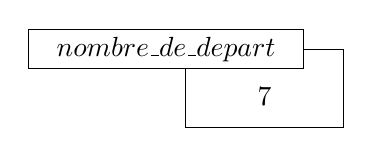
\begin{tikzpicture}
\draw (0,0)--(2,0);
\draw (2,0)--(2,1);
\draw (2,1)--(1.5,1);
\draw (0,0.75)--(0,0);
\draw (1,0.4) node {$7$};
\draw (-2,1.25)--(1.5,1.25);
\draw (1.5,1.25)--(1.5,0.75);
\draw (-2,0.75)--(1.5,0.75);
\draw (-2,0.75)--(-2,1.25);
\draw (-0.25,1) node {$nombre\_de\_depart$}; 
\end{tikzpicture}
\\
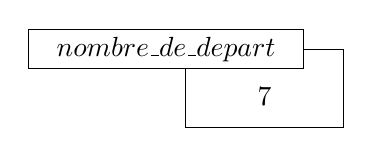
\begin{tikzpicture}
\draw (0,0)--(2,0);
\draw (2,0)--(2,1);
\draw (2,1)--(1.5,1);
\draw (0,0.75)--(0,0);
\draw (1,0.4) node {$7$};
\draw (-2,1.25)--(1.5,1.25);
\draw (1.5,1.25)--(1.5,0.75);
\draw (-2,0.75)--(1.5,0.75);
\draw (-2,0.75)--(-2,1.25);
\draw (-0.25,1) node {$nombre\_de\_depart$}; 
\end{tikzpicture}
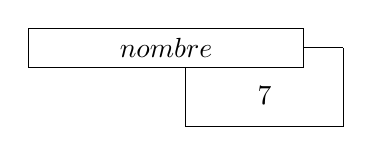
\begin{tikzpicture}
\draw (0,0)--(2,0);
\draw (2,0)--(2,1);
\draw (2,1)--(1.5,1);
\draw (0,0.75)--(0,0);
\draw (1,0.4) node {$7$};
\draw (-2,1.25)--(1.5,1.25);
\draw (1.5,1.25)--(1.5,0.75);
\draw (-2,0.75)--(1.5,0.75);
\draw (-2,0.75)--(-2,1.25);
\draw (-0.25,1) node {$nombre$}; 
\end{tikzpicture}
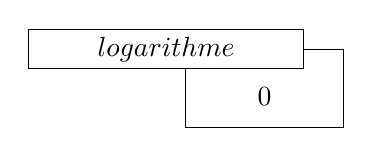
\begin{tikzpicture}
\draw (0,0)--(2,0);
\draw (2,0)--(2,1);
\draw (2,1)--(1.5,1);
\draw (0,0.75)--(0,0);
\draw (1,0.4) node {$0$};
\draw (-2,1.25)--(1.5,1.25);
\draw (1.5,1.25)--(1.5,0.75);
\draw (-2,0.75)--(1.5,0.75);
\draw (-2,0.75)--(-2,1.25);
\draw (-0.25,1) node {$logarithme$}; 
\end{tikzpicture}
\\
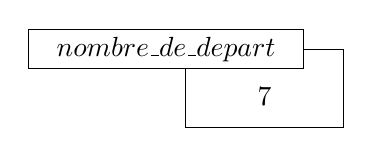
\begin{tikzpicture}
\draw (0,0)--(2,0);
\draw (2,0)--(2,1);
\draw (2,1)--(1.5,1);
\draw (0,0.75)--(0,0);
\draw (1,0.4) node {$7$};
\draw (-2,1.25)--(1.5,1.25);
\draw (1.5,1.25)--(1.5,0.75);
\draw (-2,0.75)--(1.5,0.75);
\draw (-2,0.75)--(-2,1.25);
\draw (-0.25,1) node {$nombre\_de\_depart$}; 
\end{tikzpicture}
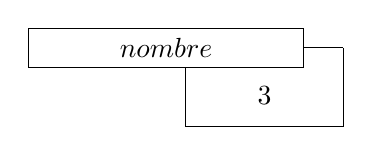
\begin{tikzpicture}
\draw (0,0)--(2,0);
\draw (2,0)--(2,1);
\draw (2,1)--(1.5,1);
\draw (0,0.75)--(0,0);
\draw (1,0.4) node {$3$};
\draw (-2,1.25)--(1.5,1.25);
\draw (1.5,1.25)--(1.5,0.75);
\draw (-2,0.75)--(1.5,0.75);
\draw (-2,0.75)--(-2,1.25);
\draw (-0.25,1) node {$nombre$}; 
\end{tikzpicture}
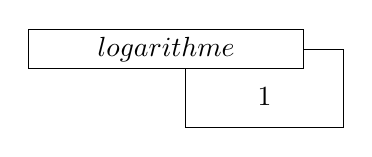
\begin{tikzpicture}
\draw (0,0)--(2,0);
\draw (2,0)--(2,1);
\draw (2,1)--(1.5,1);
\draw (0,0.75)--(0,0);
\draw (1,0.4) node {$1$};
\draw (-2,1.25)--(1.5,1.25);
\draw (1.5,1.25)--(1.5,0.75);
\draw (-2,0.75)--(1.5,0.75);
\draw (-2,0.75)--(-2,1.25);
\draw (-0.25,1) node {$logarithme$}; 
\end{tikzpicture}
\\
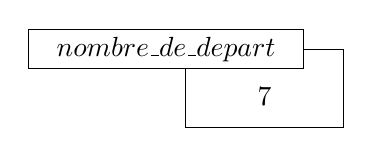
\begin{tikzpicture}
\draw (0,0)--(2,0);
\draw (2,0)--(2,1);
\draw (2,1)--(1.5,1);
\draw (0,0.75)--(0,0);
\draw (1,0.4) node {$7$};
\draw (-2,1.25)--(1.5,1.25);
\draw (1.5,1.25)--(1.5,0.75);
\draw (-2,0.75)--(1.5,0.75);
\draw (-2,0.75)--(-2,1.25);
\draw (-0.25,1) node {$nombre\_de\_depart$}; 
\end{tikzpicture}
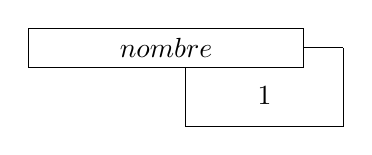
\begin{tikzpicture}
\draw (0,0)--(2,0);
\draw (2,0)--(2,1);
\draw (2,1)--(1.5,1);
\draw (0,0.75)--(0,0);
\draw (1,0.4) node {$1$};
\draw (-2,1.25)--(1.5,1.25);
\draw (1.5,1.25)--(1.5,0.75);
\draw (-2,0.75)--(1.5,0.75);
\draw (-2,0.75)--(-2,1.25);
\draw (-0.25,1) node {$nombre$}; 
\end{tikzpicture}
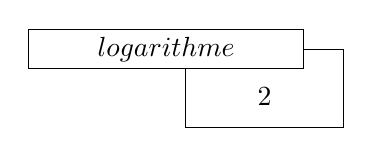
\begin{tikzpicture}
\draw (0,0)--(2,0);
\draw (2,0)--(2,1);
\draw (2,1)--(1.5,1);
\draw (0,0.75)--(0,0);
\draw (1,0.4) node {$2$};
\draw (-2,1.25)--(1.5,1.25);
\draw (1.5,1.25)--(1.5,0.75);
\draw (-2,0.75)--(1.5,0.75);
\draw (-2,0.75)--(-2,1.25);
\draw (-0.25,1) node {$logarithme$}; 
\end{tikzpicture}

Le programme s'arrête alors car la condition \textit{nombre>1} n'est plus vérifiée.

\end{minipage}
 
\begin{Exercise}[title={Evolution},counter={exo}]
 
 Pourquoi définir $2$ variables \textit{nombre\_de\_depart} et \textit{nombre}  dans le programme \ref{premcode}?
\end{Exercise}

\begin{Exercise}[title={Limites du programme},counter={exo}]
Tester le programme \ref{premcode} pour différentes valeurs de \textit{nombre\_de\_depart}. Pour quelles valeurs le résultat est il celui attendu?\\
\end{Exercise}

On observe que ce programme répète plusieurs fois la même instruction et qu'on l'a réécrite à chaque fois. On aimerait éviter d'avoir à effectuer cette réécriture et pouvoir demander à la machine, de façon concise, de répéter un certain nombre de fois un ensemble fixé d'instructions.\\
C'est le rôle des \textit{boucles}, nous allons voir qu'on peut considérer qu'il y a deux sortes de boucles.

\section{Les boucles conditionnelles}
\begin{lstlisting}[frame=lines, float=ht,caption={Première boucle \textit{while}},label=premcode2]
#Recherche du logarithme entier  
nombre_de_depart=7
nombre=nombre_de_depart
logarithme=0
while nombre>1: # si nombre<=1, la boucle arrete
    nombre=nombre//2
    logarithme=logarithme+1
print('le logarithme entier de ',nombre_de_depart,' est ',logarithme)
\end{lstlisting}

Le programme \ref{premcode2} donne une solution au problème de recherche du logarithme entier. Le mot clé \textit{while} indique à la machine qu'elle va devoir répéter un ensemble d'instructions qui suit le symbole ':' tant que la \textit{condition} est vérifiée. (c'est pour cela qu'on parle de \textit{boucle conditionnelle})\\
Afin de bien marquer le début et la fin de cet ensemble d'instructions, on décale (indente) chaque instruction de 4 espaces (ou une tabulation).\\
Tout le bloc d'instructions est décalé, par exemple dans le programme \ref{premcode2}, le bloc est constitué de deux lignes d'instructions, l'instruction \textit{print} ne fait pas partie du bloc.
On remarquera enfin la compacité du code!\\
\begin{defi}
On définit les différentes parties d'une boucles conditionnelle: on peut décomposer son code en 4 parties successives:
\begin{enumerate}
	\item \textbf{L'initialisation} dans laquelle on définit la valeur des paramètres de départ (ici \textit{logarithme} et \textit{nombre}).
	\item La définition d'une \textbf{condition de boucle} qui porte sur une (ou plusieurs) variable. (ici \textit{nombre>1})
	\item \textbf{Le bloc d'instructions} à répéter qui modifie les valeurs des paramètres et en particulier du paramètre qui sert au test. (ici \textit{nombre})
	\item \textbf{La sortie de boucle}: on doit penser à vérifier les valeurs des différents paramètres après la sortie afin qu'ils permettent de répondre à la question posée.
\end{enumerate}
\end{defi}

\begin{Exercise}[title={Construire une boucle conditionnelle},counter={exo}]
\label{exorec}
Fixer un entier $n$.\\
Calculer à l'aide d'une boucle \textit{while} le $n^{eme}$ terme de la suite définie par $u_0=1$ et pour tout $n$ de $\mathbb{N}$, $u_{n+1}=2u_n-3$. \textit{(Corrigé en fin de poly)}
\end{Exercise}

\begin{Answer}
\begin{lstlisting}[frame=lines, caption={$n^{eme}$ terme}]
#calcul du enieme terme d'une suite recurrente
a=1
n=17
while n>0:
	a=2*a-3
	n=n-1
print('Le enieme terme est ',a)  
\end{lstlisting} 
\end{Answer}

\begin{Exercise}[title={Première apparition},counter={exo}]
Charger le module random à l'aide de l'instruction \textit{import random as rd} On peut tirer un nombre au hasard entre $1$ et $6$ à l'aide de l'instruction \textit{rd.randint(1,6)}. Faire des tirages successifs jusqu'à tirer un $-$ et afficher le nombre de tirages qui ont été nécessaires. 
\end{Exercise}

\begin{Exercise}[title={Construire une boucle conditionnelle sans utiliser de compteur: division naïve},counter={exo}]
\label{exonaif}
  Soit deux nombres entiers $a$ et $b$ strictement positifs (on les choisit), construire une boucle conditionnelle qui renvoie le résultat de la division euclidienne de $a$ par $b$ en soustrayant $b$ de $a$ autant de fois que nécessaire. \textit{(Corrigé en fin de poly)}
\end{Exercise}

\begin{Answer}
\begin{lstlisting}[frame=lines, caption={division naïve}, label=premcode4]
#On divise a par b
a=67
b=7
dividende=a
quotient=0
while dividende>b:
    #on continue tant que c'est plus grand que b 
    quotient=quotient+1
    dividende=dividende-b
\end{lstlisting} 
\end{Answer}

On observe que dans le corrigé de l'exercice \label{exonaif} le dividende n'est pas exactement un compteur, c'est seulement un \emph{entier positif strictement décroissant}. Les boucles précédentes sont des boucles conditionnelles (elles répètent les instructions tant que la condition de boucle est vérifiée), il existe aussi des boucles inconditionnelles.

\section{Boucles inconditionnelles}
Dans cette section, nous allons commencer par donner une version de chacun des exemples précédents traités maintenant à l'aide d'une boucle inconditionnelle (i.e. à base de \textit{for}).


\begin{lstlisting}[frame=lines, float=ht,caption={calcul du enieme terme d'une suite recurrente version \textit{for}},label=premcode5]
a=1
n=17
for i in range(n):
	a=2*a-3
print('Le enieme terme est ',a)  
\end{lstlisting}

% \begin{verbatim}
% #calcul du enieme terme d'une suite recurrente
% #(version "for")
% a=1
% n=17
% for i in range(n):
% 	a=2*a-3
% print('Le enieme terme est ',a)
% \end{verbatim}



On remarque dans ce premier exemple (programme \ref{premcode5}) que l'on sait dès le départ le nombre de fois ($17$) qu'on veut répéter l'instruction centrale $a=2a-3$.\\
Ce n'est pas le cas dans les deux programmes \ref{premcode2} et \ref{premcode4} dans lesquels on peut majorer ou calculer ce nombre mais où il n'est pas donné \textit{a priori}.

\begin{Exercise}[title={Evolution},counter={exo}]
  Dessiner l'évolution des états des variables du programme \ref{premcode5}.
\end{Exercise}

\begin{lstlisting}[frame=lines, float=ht,caption={logarithme V2 \textit{for}},label=premcode6]
#Recherche du logarithme entier version 2 
nombre_de_depart=7
nombre=nombre_de_depart
logarithme=0
for i in range(nombre_de_depart):
    nombre=nombre//2
    if nombre>0:
        logarithme=logarithme+1   
print('le logarithme entier de ',nombre_de_depart,' est ',logarithme)
\end{lstlisting}


\begin{Exercise}[title={Evolution},counter={exo}]
  Dessiner l'évolution des états des variables du programme \ref{premcode6}.
\end{Exercise}

On remarque qu'avec cette version (programme \ref{premcode6}), on doit tout de même faire autant de tests qu'avec une boucle \textit{while} (programme \ref{premcode2}).
D'autre part, il y a beaucoup de calculs inutiles car la valeur finale de \textit{logarithme} est atteinte bien avant que le compteur $i$ n'atteigne la valeur maximale $nombre\_de\_depart-1$. Pour ce problème il semble qu'une boucle \textit{while} soit mieux adaptée.

\begin{lstlisting}[frame=lines, float=ht,caption={division euclidienne V2  \textit{for}},label=premcode7]
#Recherche de la  division de a par b
a=67
b=5
dividende=a
quotient=0
for i in range(a):
    dividende=dividende-b
    if dividende>0:
    	#on continue tant que le reste est non nul 
        quotient=i     
print('le quotient est ',quotient+1,' le reste est ',a-(quotient+1)*b)
\end{lstlisting}

\begin{Exercise}[title={Evolution},counter={exo}]
  Dessiner l'évolution des états des variables du programme \ref{premcode7}. Expliquer la présence du $+1$ dans l'expression du quotient.
\end{Exercise}

\begin{defi}
On peut décomposer le code d'une boucle \textit{for} en 4 parties successives:
\begin{enumerate}
    \item Le choix d'une variable de \textbf{compteur}. 
	\item La détermination du \textbf{domaine} décrit par ce compteur.
	\item Le \textbf{bloc d'instructions à répéter}.
	\item La \textbf{sortie de boucle}: on doit penser à vérifier les valeurs des différents paramètres après la sortie afin qu'ils permettent de répondre au problème posé.
Dans ces trois exemples (programmes \ref{premcode5}, \ref{premcode6} et \ref{premcode7}) de boucles "inconditionnelles", le compteur n'apparait pas dans les instructions.
\end{enumerate}
\end{defi}

\begin{Exercise}[title={Somme de termes},counter={exo}]
  Calculer la somme des 10 premiers entiers naturels plus grands ou égaux à 2 en utilisant une boucle \textit{for}
\end{Exercise}

\begin{lstlisting}[frame=lines, float=ht,caption={Somme de carrés  \textit{while}},label=premcode8]
#Somme des carres des nombres de 2 a 11
somme=0
#On initialise la valeur de depart de somme
for i in range(2,11+1):
    somme=somme+i**2
print('la somme des carres de 2 a 11 est ',somme)
\end{lstlisting}

Que penser du terme $11+1$ qui intervient dans \textit{range}?
Le compteur intervient il davantage dans les instructions qu'il ne le faisait dans les exemples précédents?

\section{Résumé}
Une boucle sert à faire exécuter de façon répétitive un ensemble d'instructions.
On peut connaître d'avance le nombre d'itérations à effectuer et on utilise alors plutôt une boucle \textit{for}. 
Le nombre d'itération peut aussi dépendre d'une variable qui \textit{évolue} au cours des itérations, on utilise alors plutôt une boucle \textit{while}\\
Dans une boucle le compteur peut ou non intervenir dans les instructions.\\

\textbf{Remarque1:}
On pourrait montrer qu'un programme écrit à l'aide de \textit{while} peut s'écrire à l'aide de \textit{for} et de tests \textit{if..else} (et réciproquement).\\

\textbf{Remarque2:}
Le compteur d'une boucle \textit{for} n'est pas forcément un entier, on verra des compteurs qui décrivent par exemple des chaines de caractères dans les chapitres suivants.

\section{Complexité}
Un programme écrit à l'aide de boucles répète un certains nombre de fois une ou plusieurs instructions. Il est important de pouvoir prévoir l'ordre de grandeur du temps de calcul nécessaire à l'exécution du programme. On parle de \textit{complexité en temps de calcul}.\\
\\
Pour le programme \ref{premcode4} (Division naïve), la boucle se répètera de l'ordre de $\frac{a}{b}$ fois (en réalité, c'est la partie entière de ce nombre) et il y a deux opérations par boucle (une addition et une multiplication) plus le test de comparaison du dividende, au total il y aura donc $3\frac{a}{b}$ opérations. Si on fixe $b$ et qu'on utilise ce programme pour diverses valeus de $a$ on dira que la complexité (en temps de calcul) est de l'ordre d'une constante fois $a$. On parle d'une complexité en $O(a)$. On parle aussi de complexité linéaire.\\
\\
Pour le programme \ref{premcode7} il y a un test et une opération par boucle, mais il y a $a$ boucles. La complexité en temps est de l'ordre de $2a$. C'est encore une complexité en $O(a)$. \\
\\
Pour le programme \ref{premcode2} il y a deux opérations et un test par boucle. Le nombre $n$ de boucles est tel que $2^n$ est à peu près égal au \textit{nombre\_de\_depart}. La complexité est donc de l'ordre d'une constante fois $\ln(nombre\_de\_depart)$. On a une complexité (en temps) en $O(\ln(nombre\_de\_depart))$.\\
\\
La complexité n'est pas toujours facile à déterminer. Voir par exemple le programme \ref{premcode12}. 
    

\section{Thèmes}
\begin{Exercise}[counter={exo}]
\label{sommediv} 
Écrire un code qui donne la somme de tous les diviseurs plus grands que 1 (y compris lui-même) d'un entier $n\geq2$
\end{Exercise}

\begin{Answer}
\begin{lstlisting}[frame=lines, caption={somme des diviseurs},label=premcode12]
#recherche de la somme des diviseurs d'un entier n
n=17
#initialisation de la somme
somme=0
for i in range(1,n):
	if (n%i)==0:
		somme=somme+i
print(somme)
\end{lstlisting} 
\end{Answer}

\begin{Exercise}[counter={exo},label=ppd] Écrire un code qui donne le plus petit diviseur $\geq2$ d'un entier $n$
\end{Exercise}

\begin{Answer}[ref=ppd]
\begin{lstlisting}[frame=lines, caption={plus petit diviseur},label=premcode13]
#recherche du plus petit diviseur non trivial d'un entier n
n=17
i=2
while not(n%i==0):
	i=i+1
print(i)
\end{lstlisting} 
\end{Answer}

\begin{Exercise}[title={analyse},counter={exo}]
  Pour les deux exercices précédents, identifier le compteur, préciser si la boucle est conditionnelle, identifier la condition éventuelle de boucle.\\
 \end{Exercise}
 
\section{Boucles imbriquées}

Trouver à quels problèmes répondent les boucles des programmes \ref{premcode14}, \ref{premcode15}, \ref{premcode16} et \ref{premcode17}. 


\begin{lstlisting}[frame=lines, caption={ boucles imbriquées}, label=premcode14]
for i in range (27):
    j=3
	k=i
	while k>1 and j>0:
		k=k-1
		if(i%k)==0:
			j=j-1
			print(i)		
\end{lstlisting}

\begin{lstlisting}[frame=lines, caption={boucles imbriquées},label=premcode15]
nombre=8
n=nombre
while n>0:
    n=n-1
    a=0
	for i in range(nombre)
	    a=a+i
	print(a)    
\end{lstlisting} 

\begin{lstlisting}[frame=lines,  caption={boucles imbriquées},label=premcode16]
nombre=8
for i in range(nombre):
	for j in range(nombre):
		print(i,j**2) 
\end{lstlisting} 

\begin{lstlisting}[frame=lines, caption={boucles imbriquées},label=premcode17]
nombre=8
for j in range(nombre):
	for i in range(nombre):
		print(i,j**2) 
\end{lstlisting} 

\section{Solutions}
\shipoutAnswer



%%% Local Variables: 
%%% mode: latex
%%% TeX-master: "cours-ipt"
%%% End: 

